%%%%%%%%%%%%%%%%%%%%%%%%%%%%%%%%%%%%%%%%%%%%%%%%%%%%%%%%%%%%%%%%%%%%%%
% Problem statement
\begin{statement}[
  problempoints=100,
  timelimit=2 seconds,
  memorylimit=512 MiB,
]{Bolivija}

Bolivia, a beautiful South American country rich in culture and history, 
is filled with natural wonders, including parts of the Amazon rainforest and the Andes mountain range.  
More importantly for our contestants, it will be the host of the next International Olympiad in Informatics!

As part of promoting the competition, the organizers have been tasked with 
photographing the mountain range and creating an album of the most breathtaking images.  
The mountain range is represented as an array $v$ of $N$ non-negative integers, 
where $v_i$ denotes the height of the $i$-th mountain.  
It is guaranteed that $N$ is odd and that the tallest mountain — located at position $\frac{N+1}{2}$ — 
is the extinct volcano Nevado Sajama.

The organizers have very specific conditions for the photographs.  
First, they choose two non-negative integers $A$ and $B$ such that $A < B$ and $B$ 
is less than or equal to the height of Nevado Sajama.  
They then adjust the camera so that the width of the photograph captures all $N$ mountains, 
but only the vertical range between $A$ and $B$.  
Additionally, the organizers are satisfied with a photograph only if it is symmetric 
with respect to the vertical axis passing through the central mountain.

\begin{figure}[!h]
      \centering
      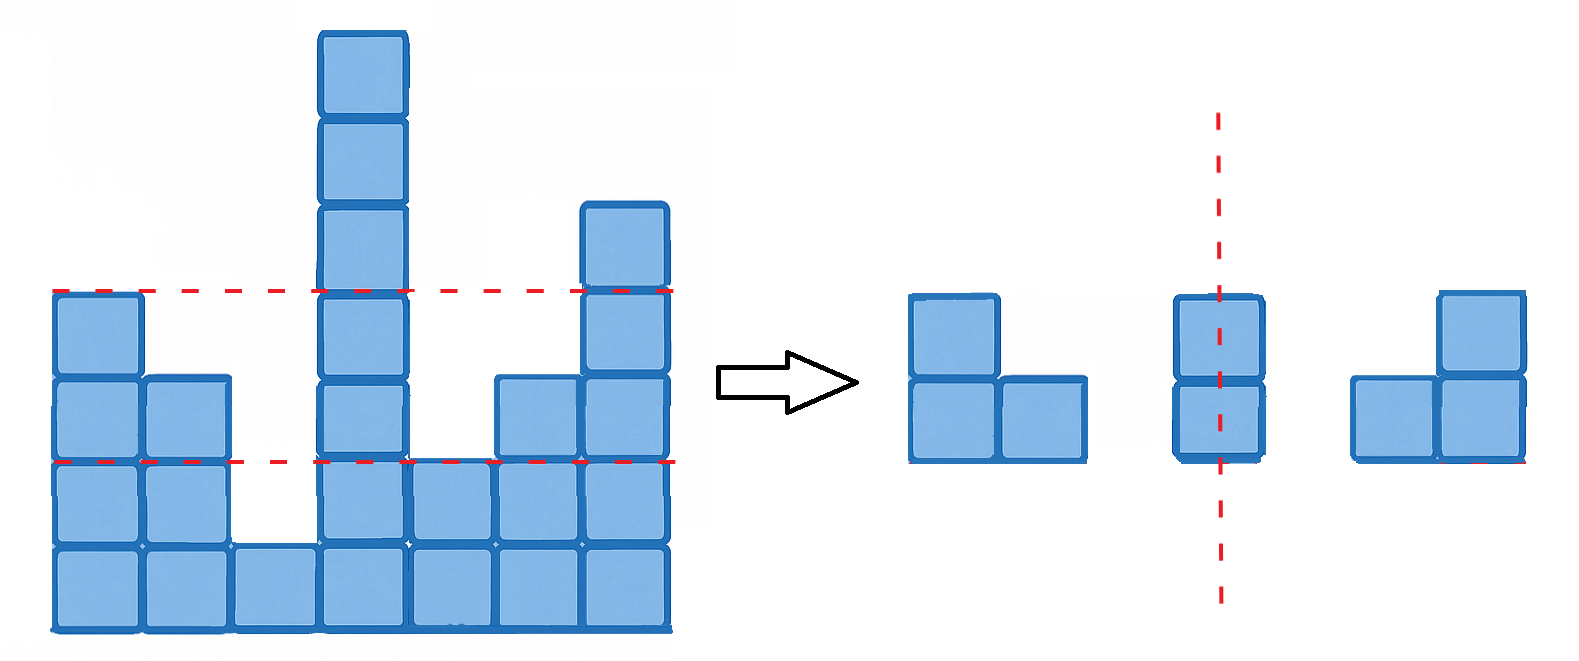
\includegraphics[width=\linewidth]{pic/planine.png}
      \caption*{Illustration: Example of a valid photo selection corresponding to the second sample case}
\end{figure}

The organizers now want to know how many different photographs they can take — that is,  
how many pairs $(A, B)$ satisfy the given conditions.  
While thinking too long about the answer, intense tectonic activity 
caused the heights of some mountains to change.  
A total of $Q$ height changes occur, and your task is to help the organizers 
determine the number of valid photographs after each change.  
Importantly, none of the changes affects the height of the central mountain, 
and it always remains the tallest mountain.

%%%%%%%%%%%%%%%%%%%%%%%%%%%%%%%%%%%%%%%%%%%%%%%%%%%%%%%%%%%%%%%%%%%%%%
% Input
\subsection*{Input}

The first line contains two natural numbers $N$ and $Q$, representing 
the number of mountains and the number of height changes.

The second line contains an array $v$ of $N$ non-negative integers, 
the heights of the mountains in order.  
It is guaranteed that $N$ is odd and that the central mountain is the tallest.

Each of the next $Q$ lines contains two non-negative integers $x_i$ and $h_i$ ($1 \leq x_i \leq N$), 
indicating that the height of the mountain at position $x_i$ changes to $h_i$.  
It is guaranteed that $x_i \neq \frac{N+1}{2}$ and that the new height is less than or equal to 
the height of the central mountain.

%%%%%%%%%%%%%%%%%%%%%%%%%%%%%%%%%%%%%%%%%%%%%%%%%%%%%%%%%%%%%%%%%%%%%%
% Output
\subsection*{Output}

Print $Q + 1$ lines.  
In the $i$-th line, print the number of valid photographs after the first $i-1$ height changes.

%%%%%%%%%%%%%%%%%%%%%%%%%%%%%%%%%%%%%%%%%%%%%%%%%%%%%%%%%%%%%%%%%%%%%%
% Scoring
\subsection*{Scoring}

In all subtasks, it holds that $3 \leq N \leq 200\,000$ and $0 \leq Q \leq 200\,000$.

For all $i = 1, \dots, N$, it holds that $v_i \leq 654\,200$ 
(the height of Nevado Sajama in centimeters).

{\renewcommand{\arraystretch}{1.4}
  \setlength{\tabcolsep}{6pt}
  \begin{tabular}{ccl}
   Subtask & Points & Constraints \\ \midrule
    1 & 9 & $Q = 0$, $N \leq 300$, and $v_i \leq 300$ for all $i = 1, \dots, N$ \\
    2 & 23 & $Q = 0$ \\
    3 & 31 & Each change modifies a mountain's height by at most $1$. \\
    4 & 37 & No additional constraints. \\
\end{tabular}}

%%%%%%%%%%%%%%%%%%%%%%%%%%%%%%%%%%%%%%%%%%%%%%%%%%%%%%%%%%%%%%%%%%%%%%
% Sample Cases
\subsection*{Sample Cases}
\begin{tabularx}{\textwidth}{X'X'X}
\sampleinputs{test/bolivija.dummy.in.1}{test/bolivija.dummy.out.1} &
\sampleinputs{test/bolivija.dummy.in.2}{test/bolivija.dummy.out.2} &
\sampleinputs{test/bolivija.dummy.in.3}{test/bolivija.dummy.out.3}
\end{tabularx}

\textbf{Explanation of the Second Sample Case:}

The valid choices for $(A, B)$ are:  
$(0, 1), (2, 3), (2, 4), (3, 4), (5, 6), (5, 7), (6, 7)$.  
There are a total of seven pairs.

The figure above corresponds to the choice $A = 2$ and $B = 4$.

%%%%%%%%%%%%%%%%%%%%%%%%%%%%%%%%%%%%%%%%%%%%%%%%%%%%%%%%%%%%%%%%%%%%%%
% We're done
\end{statement}
